\documentclass{ximera}

\newcommand{\RR}{\mathbb R}
\renewcommand{\d}{\,d}
\newcommand{\dd}[2][]{\frac{d #1}{d #2}}
\renewcommand{\l}{\ell}
\newcommand{\ddx}{\frac{d}{dx}}
\newcommand{\dfn}{\textbf}
\newcommand{\eval}[1]{\bigg[ #1 \bigg]}


\outcome{Identify real numbers.}
\outcome{Compute the distance between points.}
\outcome{Find the equations for planes.}
\outcome{Give the equation for a circle.}
\outcome{Give the equation for a sphere or ball.}

\title[Dig-In:]{Working in two and three dimensions}

\begin{document}
\begin{abstract}
  We talk about basic geometry in higher dimensions.
\end{abstract}
\maketitle


The word \textit{geometry} can be broken into \textit{geo} meaning
``world'' and \textit{metry} meaning ``measure.'' In this section we
will tell you what our mathematical ``world'' is, and how we ``measure''
it.

\section{Higher dimensions}

In our previous courses, we studied functions where the input was a
single real number and the output was a single real number. Note, the
word ``real'' is being used in a technical sense:

\begin{definition}
  A \dfn{real number} is a number that has a (possibly infinite)
  decimal representation. The set of all real numbers is denoted by
  $\R$.
\end{definition}
\begin{question}
  Which of the following are real numbers?
  \begin{selectAll}
    \choice[correct]{$\sqrt{7}$}    
    \choice[correct]{$0$}
    \choice[correct]{$-3$}
    \choice[correct]{$\pi$}
    \choice[correct]{$e$}
    \choice{$x$}
    \choice{$\sqrt{-1}$}
    \choice{$\infty$}
  \end{selectAll}
\end{question}

When we say a function maps a real number to a real number, we write:
\[
f:\R\to \R
\]
When working in two dimensions, we need a way of talking about ordered
pairs of numbers. We denote the set of all ordered pairs of real
numbers by $\R^2$. When working in three dimensions we denote the set
of all ordered triples of real numbers by $\R^3$.  In three dimensions
we have three coordinates axes, the $x$-axis, $y$-axis, and $z$-axis:
\begin{image}[1in]
\begin{tikzpicture}
  \draw[->] (-1,0)--(1,0);
  \draw[->] (0,-1)--(0,1);
  \draw[->] (.4,.7)--(-.4,-.7);
  \node[right] at (1,0) {$x$};
  \node[above] at (0,1) {$y$};
  \node[below] at (-.4,-.7) {$z$};
\end{tikzpicture}
\end{image}
The axes point according to the \dfn{right-hand-rule}:
\begin{image}[2in]
  %% Based on: https://commons.wikimedia.org/wiki/File:Right_hand_rule_cross_product.svg
  %% Which was based on: https://commons.wikimedia.org/wiki/File:Right_hand_cross_product.png
  %% Which was based on: https://commons.wikimedia.org/wiki/File:LeftHandOutline.png
  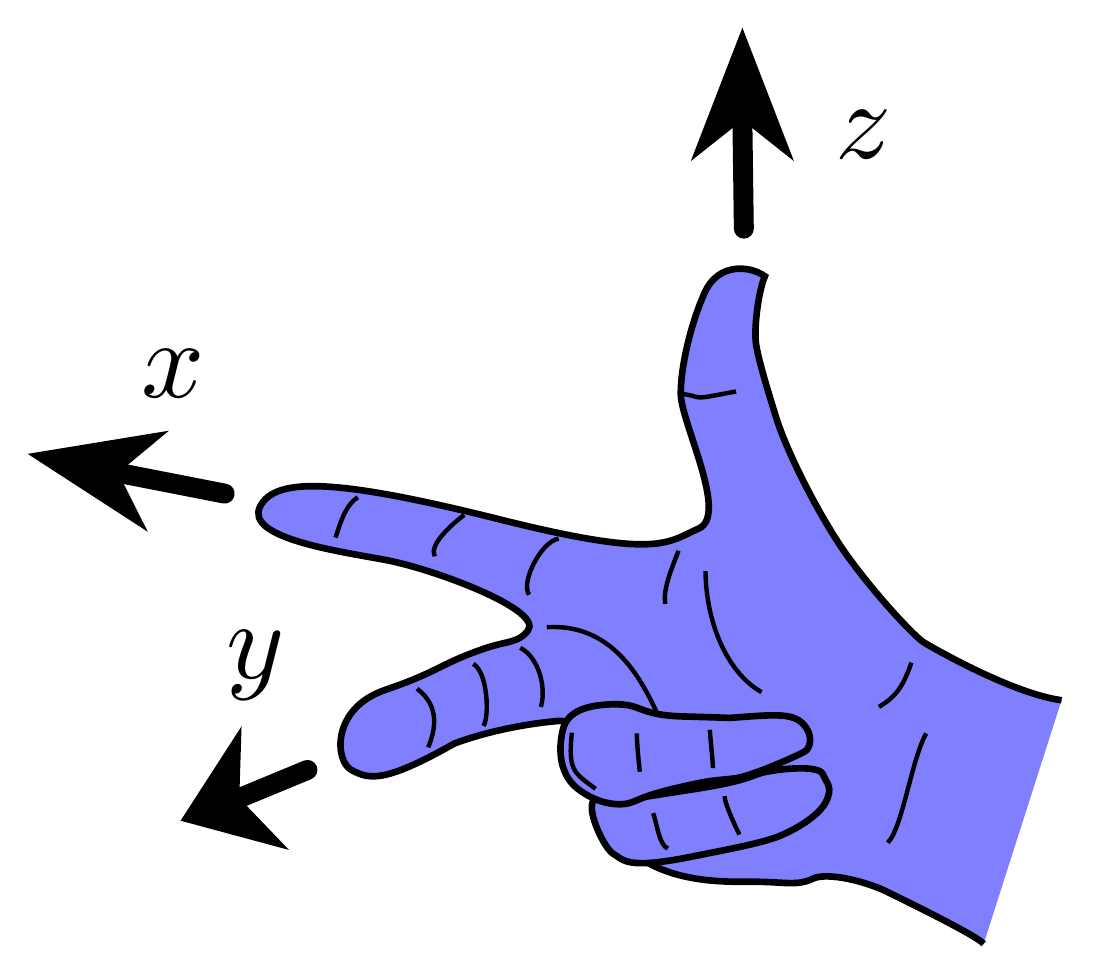
\begin{tikzpicture}[y=0.80pt, x=0.80pt, yscale=-1.000000, xscale=1.000000, inner sep=0pt, outer sep=0pt]
    \path[draw=black,fill=blue!50!white,line width=2.400pt] (466.9820,303.7880) ..
    controls (444.9820,300.7880) and (409.9820,280.7880) .. (404.9820,277.7880) ..
    controls (399.9820,274.7880) and (376.9820,249.7880) .. (364.9820,230.7880) ..
    controls (352.9820,211.7880) and (341.9820,188.7880) .. (337.9820,175.7880) ..
    controls (333.9820,162.7880) and (329.9820,149.7880) .. (328.9820,142.7880) ..
    controls (327.9820,135.7880) and (329.9820,119.2880) .. (332.9820,112.2880) ..
    controls (325.9820,107.2880) and (311.9820,106.2880) .. (305.9820,119.2880) ..
    controls (299.9820,132.2880) and (294.9820,152.2880) .. (294.9820,165.2880) ..
    controls (294.9820,178.2880) and (316.9820,220.2880) .. (302.9820,226.2880) ..
    controls (288.9820,232.2880) and (285.9820,240.2880) .. (213.9820,222.2880) ..
    controls (141.9820,204.2880) and (111.9820,202.2880) .. (104.9820,216.2880) ..
    controls (97.9820,230.2880) and (138.9820,236.2880) .. (160.9820,240.2880) ..
    controls (182.9820,244.2880) and (233.0030,262.9220) .. (225.9820,272.2880) ..
    controls (221.6320,278.0900) and (216.6070,276.7760) .. (205.2730,280.7760) ..
    controls (185.6620,287.6980) and (185.9650,290.7420) .. (161.4820,299.1210) ..
    controls (137.0490,307.4830) and (138.6390,331.3470) .. (146.3150,335.3510) ..
    controls (153.9910,339.3550) and (160.3310,341.6930) .. (192.7010,323.3380) ..
    controls (207.0510,317.9980) and (224.4830,314.4530) .. (239.8160,313.1200) ..
    controls (255.1490,311.7870) and (264.4840,369.1200) .. (281.1500,377.7870) ..
    controls (297.8160,386.4540) and (317.1490,385.7870) .. (329.1490,385.7870) ..
    controls (341.1490,385.7870) and (347.8150,387.7880) .. (354.4820,384.4540) ..
    controls (361.1490,381.1200) and (379.8160,385.7860) .. (389.8160,391.1200) ..
    controls (389.8160,391.1200) and (428.4830,409.7870) .. (431.8160,413.7870);
    \path[draw=black,line width=1.600pt] (234.4830,270.7870) .. controls
    (268.4820,268.7880) and (280.4820,301.4540) .. (288.4820,318.7880);
    \path[draw=black,line width=1.600pt] (306.1490,245.4530) .. controls
    (306.4830,270.7870) and (317.1500,292.1210) .. (331.4820,300.1190);
    \path[draw=black,line width=1.600pt] (239.8160,230.7870) .. controls
    (231.8160,232.1200) and (222.4830,250.7870) .. (226.4830,256.1200);
    \path[draw=black,line width=1.600pt] (197.1490,220.1200) .. controls
    (191.8160,224.1200) and (181.1490,233.4530) .. (183.8160,238.7870);
    \path[draw=black,line width=1.600pt] (149.1490,212.1200) .. controls
    (142.4820,216.1200) and (140.3150,227.6210) .. (138.9820,230.2870);
    \path[draw=black,line width=1.600pt] (222.4830,280.1210) .. controls
    (230.4830,284.1210) and (234.4830,297.4530) .. (231.8160,306.7870);
    \path[draw=black,line width=1.600pt] (201.2960,287.3930) .. controls
    (207.9630,291.3930) and (208.5440,311.3860) .. (205.8770,315.3860);
    \path[draw=black,line width=1.600pt] (175.8480,298.5900) .. controls
    (184.4960,305.0750) and (185.4390,314.1240) .. (180.9370,325.0560);
    \path[draw=black,line width=1.600pt] (293.9820,236.2880) .. controls
    (289.9820,246.2880) and (286.9820,254.2880) .. (287.9820,260.2880);
    \path[draw=black,line width=1.600pt] (294.9820,165.2880) .. controls
    (306.9290,166.9950) and (297.6590,168.5400) .. (319.9820,164.2880);
    \path[draw=black,line width=1.600pt] (399.1490,286.7880) .. controls
    (395.1490,298.7880) and (391.1490,302.7870) .. (384.4820,306.7870);
    \path[draw=black,fill=blue!50!white,line width=2.400pt] (299.8160,374.4550) ..
    controls (315.7210,371.2740) and (327.1500,369.1220) .. (335.8160,366.4550) ..
    controls (344.4820,363.7880) and (357.1480,356.4540) .. (360.4820,349.7880) ..
    controls (363.8160,343.1220) and (361.1490,341.7890) .. (359.1490,337.1220) ..
    controls (357.1490,332.4550) and (335.1500,335.1220) .. (329.8160,337.1220) ..
    controls (324.4820,339.1220) and (319.8160,341.1220) .. (297.8160,344.4550) ..
    controls (275.8160,347.7880) and (269.8160,349.4550) .. (258.4820,348.1210) ..
    controls (249.1900,347.0270) and (259.8170,370.4540) .. (264.4830,373.1210) ..
    controls (269.1490,375.7880) and (269.8160,380.4550) .. (299.8160,374.4550) --
    cycle;
    \path[draw=black,fill=blue!50!white,line width=2.400pt] (316.7840,311.7880) ..
    controls (335.6810,310.4550) and (345.1320,309.1220) .. (350.2190,314.4550) ..
    controls (355.3060,319.7880) and (353.1250,325.1220) .. (351.6720,326.4550) ..
    controls (350.2190,327.7880) and (333.5010,335.1210) .. (324.7790,337.7880) ..
    controls (316.0560,340.4550) and (314.6030,338.4550) .. (297.1600,342.4550) ..
    controls (279.7160,346.4550) and (278.2630,347.7880) .. (273.1740,349.7880) ..
    controls (268.0860,351.7880) and (257.9110,351.1210) .. (248.4630,343.7880) ..
    controls (239.0140,336.4550) and (240.4670,323.7880) .. (241.1940,319.7880) ..
    controls (241.9210,315.7880) and (242.6490,307.1210) .. (260.8190,305.7880) ..
    controls (278.9890,304.4550) and (273.1730,310.4540) .. (296.4330,311.1210) ..
    controls (319.6910,311.7880) and (316.7840,311.7880) .. (316.7840,311.7880) --
    cycle;
    \path[draw=black,line width=1.600pt] (245.8150,318.4550) .. controls
    (243.8920,335.7600) and (246.9240,336.6210) .. (256.4820,343.7880);
    \path[draw=black,line width=1.600pt] (275.1490,318.7870) .. controls
    (275.1490,324.1200) and (276.4820,336.1200) .. (276.4820,336.1200);
    \path[draw=black,line width=1.600pt] (308.1490,317.1200) .. controls
    (308.1490,319.7870) and (309.4830,330.4530) .. (309.4830,334.4530);
    \path[draw=black,line width=1.600pt] (314.8150,347.1220) .. controls
    (314.8150,351.1220) and (321.4820,364.4550) .. (321.4820,364.4550);
    \path[draw=black,line width=1.600pt] (282.4820,354.7880) .. controls
    (283.8150,357.4550) and (285.1490,369.4540) .. (289.1490,370.7880);
    \path[draw=black,line width=1.600pt] (405.8150,318.7880) .. controls
    (399.1490,330.7880) and (395.1490,361.4560) .. (388.4820,368.1220);
    \path[draw=black,fill=black,line cap=round,line width=7.200pt]
    (323.4820,90.7880) -- (322.8140,41.7880);
    \path[fill=black] (322.8140,41.7880) -- (299.5010,60.3000) -- (322.8140,0.0000)
    -- (346.1270,60.3000) -- cycle;
    \path[draw=black,fill=black,line cap=round,line width=7.200pt]
    (88.9960,210.4600) -- (40.9000,201.0670);
    \path[fill=black] (40.9000,201.0670) -- (54.2400,227.6800) -- (0.0000,192.5000)
    -- (63.7990,182.0440) -- cycle;
    \path[draw=black,fill=black,line cap=round,line width=7.200pt]
    (126.3770,335.2550) -- (95.5850,348.0050);
    \path[fill=black] (95.5850,348.0050) -- (118.0640,371.4130) --
    (69.0630,358.1970) -- (96.6050,315.5680) -- cycle;
    \path[fill=black,line join=miter,line cap=butt,line width=0.800pt]
    (51.2201,166.8365) node[above right] (text4204) {\scalebox{4}{$x$}};
    \path[fill=black,line join=miter,line cap=butt,line width=0.800pt]
    (89.7117,303.4817) node[above right] (text4208) {\scalebox{4}{$y$}};
    \path[fill=black,line join=miter,line cap=butt,line width=0.800pt]
    (364.9268,59.0600) node[above right] (text4212) {\scalebox{4}{$z$}};
  \end{tikzpicture}
\end{image}
Of course you will need to ``spin'' your hand around to align your
pointer-finger with the $x$-axis and your middle-finger with the
$y$-axis. Then your thumb will point in the $z$-direction.
\begin{question}
  Which of the following axes are aligned according to the right-hand rule?
  \begin{hint}
    Point the ``pointer finger'' of your right hand in the positive
    direction of the $x$-axis while simultaneously pointing your
    ``middle finger'' in the positive direction of the $y$-axis. Your
    thumb will point in the positive direction of the $z$-axis.
  \end{hint}
   \begin{selectAll}
     \choice[correct]{
       \begin{tikzpicture}[baseline=2ex]
         \draw[->] (-1,0)--(1,0);
         \draw[->] (0,-1)--(0,1);
         \draw[->] (.4,.7)--(-.4,-.7);
         \node[right] at (1,0) {$y$};
         \node[above] at (0,1) {$z$};
         \node[below] at (-.4,-.7) {$x$};
     \end{tikzpicture}}
     \choice{
       \begin{tikzpicture}[baseline=2ex]
         \draw[->] (-1,0)--(1,0);
         \draw[->] (0,-1)--(0,1);
         \draw[->] (.4,.7)--(-.4,-.7);
         \node[right] at (1,0) {$y$};
         \node[above] at (0,1) {$x$};
         \node[below] at (-.4,-.7) {$z$};
     \end{tikzpicture}}
     \choice{
       \begin{tikzpicture}[baseline=2ex]
         \draw[->] (-1,0)--(1,0);
         \draw[->] (0,-1)--(0,1);
         \draw[->] (.4,.7)--(-.4,-.7);
         \node[right] at (1,0) {$x$};
         \node[above] at (0,1) {$z$};
         \node[below] at (-.4,-.7) {$y$};
     \end{tikzpicture}}
     \choice[correct]{
       \begin{tikzpicture}[baseline=2ex]
         \draw[->] (-1,0)--(1,0);
         \draw[->] (0,-1)--(0,1);
         \draw[->] (.4,.7)--(-.4,-.7);
         \node[right] at (1,0) {$z$};
         \node[above] at (0,1) {$x$};
         \node[below] at (-.4,-.7) {$y$};
     \end{tikzpicture}}
   \end{selectAll}
\end{question}




\section{Basic plotting}


To plot a point $(a,b,c)$ in $\R^3$, you move $a$ in the
$x$-direction, $b$ in the $y$-direction and $c$ in the $z$ direction.

\begin{image}
  \begin{tikzpicture}
    \begin{axis}[
        axis lines=none,
        clip=false,
        width=5in,
        height=2.5in,
      ]          
      \addplot [->,textColor] plot coordinates {(0,0) (-2,-4)}; %% x axis
      \addplot [->,textColor] plot coordinates {(0,0) (4,0)}; %% y axis
      \addplot [->,textColor] plot coordinates {(0,0) (0,6)}; %% z axis
      
      \addplot [dashed] plot coordinates {(-1.3,-2.6) (2.6,-2.6)}; %%bottom dashed line
      \addplot [dashed] plot coordinates {(2.6,-2.6) (3.5,0)}; %% bottom right dashed
      \addplot [dashed] plot coordinates {(3.5,0) (3.5,5.5)};  %% back right vert dashed
      \addplot [dashed] plot coordinates {(2.6,-2.6) (2.6,2.9)}; %% front right vert dashed
      \addplot [dashed] plot coordinates {(3.5,5.5) (2.6,2.9)}; %% top right dashed
      \addplot [dashed] plot coordinates {(0,5.5) (-1.3,2.9)}; %% top left dashed
      \addplot [dashed] plot coordinates {(-1.3,-2.6) (-1.3,2.9)}; %% left vert front
      \addplot [dashed] plot coordinates {(-1.3,2.9) (2.6,2.9)}; %% top horz
      \addplot [dashed] plot coordinates {(0,5.5) (3.5,5.5)}; %% top horz rear
            
      \node at (axis cs:-1.3,-2.6) [anchor=east] {$a$};          
      \node at (axis cs:3.5,0) [anchor=south west] {$b$};
      \node at (axis cs:0,5.5) [anchor=south east] {$c$};

      \addplot[penColor,only marks,mark=*] coordinates{(2.6,2.9)};  %% closed hole
      \node[penColor,below right] at (axis cs:2.6,2.9) {$(a,b,c)$};
    \end{axis}
  \end{tikzpicture}
\end{image}

Of course, we're going to be plotting many points. We typically
described groups of points, as those that satisfy a given equation
involving $x$, $y$, and $z$. Here is a place where working in three
dimensions is really different from working in two.
\begin{itemize}
\item In $\R^2$, any equation involving $x$ and/or $y$ draws a \textbf{curve}.
\item In $\R^3$, any equation involving $x$, $y$, and/or $z$ draws a \textbf{surface}.  
\end{itemize}

The most basic surface in $\R^3$ is a plane.

\begin{question}
  The $(y,z)$-plane corresponds to which of the following
  equations?
  \begin{multipleChoice}
    \choice[correct]{$x=0$}
    \choice{$y=0$}
    \choice{$z=0$}
  \end{multipleChoice}
  \begin{hint}
    For every point on the $(y,z)$-plane, the $x$-coordinate is zero.
  \end{hint}
\end{question}

\begin{question}
  Which of the following most accurately describes the solution
  set of $y=2$ in $\R^3$?
  \begin{multipleChoice}
    \choice{a horizontal line}
    \choice{a vertical line}
    \choice{a plane parallel to the $(x,y)$-plane}
    \choice[correct]{a plane parallel to the $(x,z)$-plane}
    \choice{a plane parallel to the $(y,z)$-plane}
  \end{multipleChoice}
  \begin{hint}
    $y=2$ consists of all those points where $y=2$, but $x$ and
    $z$ are allowed to be anything.  
  \end{hint}
\end{question}


Another way to think of the point $(a,b,c)$ is as the intersection of the planes $x=a$, $y=b$, $z=c$. 
\begin{onlineOnly}
  Move the point around below to see the planes that define it.
  \geogebra{KyDyU28S}{800}{600}
\end{onlineOnly}


While the intersection of three planes is a point, the intersection of
two planes is a line.

\begin{question}
  What is the intersection of the $(x,y)$-plane and the $(y,z)$-plane?
  \begin{prompt}
    \begin{multipleChoice}
      \choice{The $x$-axis.}
      \choice[correct]{The $y$-axis.}
      \choice{The $z$-axis.}
    \end{multipleChoice}
  \end{prompt}
  \begin{question}
  What is the intersection of the $(x,y)$-plane and the $(x,z)$-plane?
  \begin{prompt}
    \begin{multipleChoice}
      \choice[correct]{The $x$-axis.}
      \choice{The $y$-axis.}
      \choice{The $z$-axis.}
    \end{multipleChoice}
  \end{prompt}
  \begin{question}
    What is the intersection of the $(x,z)$-plane and the $(y,z)$-plane?
    \begin{prompt}
      \begin{multipleChoice}
        \choice{The $x$-axis.}
      \choice{The $y$-axis.}
      \choice[correct]{The $z$-axis.}
      \end{multipleChoice}
    \end{prompt}
  \end{question}
  \end{question}
\end{question}




\section{Distance and spheres}

So the objects in our geometry are made of points, and now we must
tell you how we plan to ``measure'' objects. To do this, we'll use our
old friend, the distance formula.

\begin{theorem}
  Given two points $P=(x,y)$ and $Q=(a,b)$ in $\R^2$, the distance between
  them is given by:
  \[
  |PQ|=\sqrt{(x-a)^2 + (y-b)^2}
  \]
  \begin{explanation}
    This is nothing more than a corollary of the Pythagorean
    Theorem. Plot the points $P=(a,b)$ and $Q=(x,y)$:
    \begin{image}
      \begin{tikzpicture}
	\begin{axis}[
            xmin=0, xmax=5,ymin=0,ymax=5,
            axis lines =left, 
            every axis y label/.style={at=(current axis.above origin),anchor=south},
            every axis x label/.style={at=(current axis.right of origin),anchor=west},
            xtick={1,3}, xticklabels={$a$,$x$},
            ytick={2,3}, yticklabels={$b$,$y$},
            axis on top,
          ]       
          \addplot[penColor,dashed] plot coordinates {(1,0) (1,2)};
          \addplot[penColor,dashed] plot coordinates {(0,2) (1,2)};
          \addplot[penColor,dashed] plot coordinates {(3,0) (3,3)};
          \addplot[penColor,dashed] plot coordinates {(0,3) (3,3)};
          \addplot[penColor2,only marks,mark=*] coordinates{(1,2)};  %% closed hole          
          \addplot[penColor,only marks,mark=*] coordinates{(3,3)};  %% closed hole          
        \end{axis}
      \end{tikzpicture}
    \end{image}
    We may now construct a right triangle with horizontal side length
    $\answer[given]{(x-a)}$ and vertical side length
    $\answer[given]{(y-b)}$ whose hypotenuse is the shortest path
    between the two points:
    \begin{image}
      \begin{tikzpicture}
        \begin{axis}[
            xmin=0, xmax=5,ymin=0,ymax=5,
            axis lines =left, 
            every axis y label/.style={at=(current axis.above origin),anchor=south},
            every axis x label/.style={at=(current axis.right of origin),anchor=west},
            xtick={1,3}, xticklabels={$a$,$x$},
            ytick={2,3}, yticklabels={$b$,$y$},
            axis on top,
          ]       
          \node at (axis cs:2,1.75) {$(x-a)$}; 
          \node at (axis cs:3.5,2.5) {$(y-b)$}; 
          \addplot[dashed] plot coordinates {(1,2) (3,3)};
          \addplot[textColor] plot coordinates {(1,2) (3,2)};
          \addplot[textColor] plot coordinates {(3,2) (3,3)};
          \addplot[textColor] plot coordinates {(2.83,2) (2.83,2.2) (3,2.2)};
          \addplot[penColor2,only marks,mark=*] coordinates{(1,2)};  %% closed hole          
          \addplot[penColor,only marks,mark=*] coordinates{(3,3)};  %% closed hole          
        \end{axis}
      \end{tikzpicture}
    \end{image}
    By the Pythagorean Theorem, the length of this path is given by 
    \[
    |PQ|=\sqrt{(x-a)^{2}+(y-b)^{2}}.
    \]
  \end{explanation}
\end{theorem}

\begin{question}
  What is the distance between the points $P=(-17,379)$ and
  $Q=(14,-101)$ in $\R^2$?
  \begin{prompt}
    \[
    |PQ|=\answer{481}\unit{units}.
    \]
  \end{prompt}
\end{question}

On a completely related note, what's the most famous theorem in
mathematics? I'll tell you: The Pythagorean Theorem. In essance, the
distance gformula \textit{is} The Pythagorean Theorem. Let's see if we
can explain why the Pythagorean Theorem is true.

\begin{theorem}
  Given a right triangle,
  \begin{image}
    \begin{tikzpicture}
      \coordinate (A) at (0,2);
      \coordinate (B) at (0,5);
      \coordinate (C) at (6.5,2);
      \tkzMarkRightAngle(C,A,B)
      \tkzDefMidPoint(A,B) \tkzGetPoint{a}
      \tkzDefMidPoint(A,C) \tkzGetPoint{b}
      \tkzDefMidPoint(B,C) \tkzGetPoint{c}
      \draw (A)--(B)--(C)--cycle;
      \tkzLabelPoints[above](c)
      \tkzLabelPoints[below](b)
      \tkzLabelPoints[left](a)
    \end{tikzpicture}
  \end{image}
  we have that $a^2 + b^2 = c^2.$
  \begin{explanation}
    Given a right triangle with legs $a$ and $b$, and hypotenuse $c$,
    we can make the following squares each with side length $(a+b)$:
    \begin{image}
      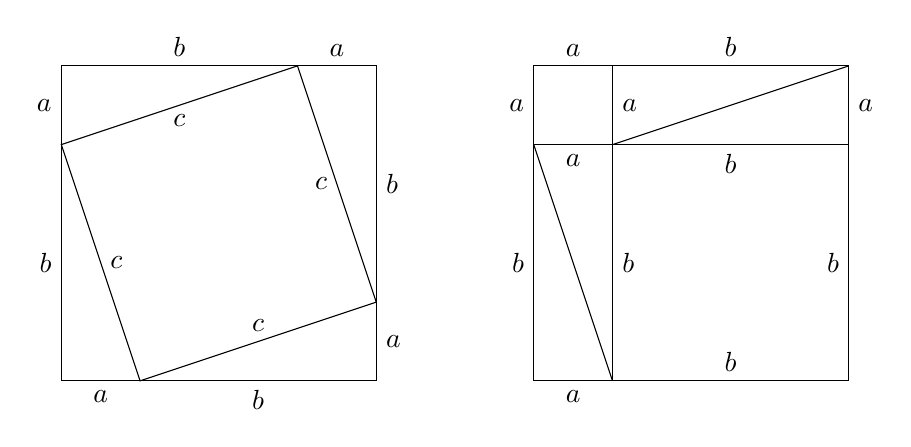
\begin{tikzpicture}
        %% First square
        \coordinate (A) at (0,0);
        \coordinate (B) at (0,4);
        \coordinate (C) at (4,4);
        \coordinate (D) at (4,0);
        \coordinate (E) at (1,0);
        \coordinate (F) at (0,3);
        \coordinate (G) at (3,4);
        \coordinate (H) at (4,1);

        \tkzMarkRightAngle(A,B,C)
        \tkzMarkRightAngle(B,C,D)
        \tkzMarkRightAngle(C,D,A)
        \tkzMarkRightAngle(D,A,B)

        \tkzMarkRightAngle(E,F,G)
        \tkzMarkRightAngle(F,G,H)
        \tkzMarkRightAngle(G,H,E)
        \tkzMarkRightAngle(H,E,F)
        
        
        \draw (A)--(B)--(C)--(D)--cycle;
        \draw (E)--(F)--(G)--(H)--cycle;
        
        \node[right] at (.5,1.5) {$c$};
        \node[above] at (2.5,.5) {$c$};
        \node[left] at (3.5,2.5) {$c$};
        \node[below] at (1.5,3.5) {$c$};

        \node[left] at (0,1.5) {$b$};
        \node[below] at (2.5,0) {$b$};
        \node[right] at (4,2.5) {$b$};
        \node[above] at (1.5,4) {$b$};

        \node[left] at (0,3.5) {$a$};
        \node[right] at (4,.5) {$a$};
        \node[below] at (.5,0) {$a$};
        \node[above] at (3.5,4) {$a$};

        %% Second square
        \coordinate (AA) at (6,0);
        \coordinate (BB) at (6,4);
        \coordinate (CC) at (10,4);
        \coordinate (DD) at (10,0);
        \coordinate (EE) at (7,0);
        \coordinate (FF) at (6,3);
        \coordinate (GG) at (7,4);
        \coordinate (HH) at (10,3);
        \coordinate (II) at (7,3);

        \tkzMarkRightAngle(II,GG,CC)
        \tkzMarkRightAngle(II,HH,CC)
        \tkzMarkRightAngle(FF,II,EE)
        \tkzMarkRightAngle(FF,AA,EE)
        
        \draw (AA)--(BB)--(CC)--(DD)--cycle;
        \draw (EE)--(FF);
        \draw (II)--(CC);
        \draw (EE)--(GG);
        \draw (FF)--(HH);
        
        \node[below] at (6.5,3) {$a$};
        \node[right] at (7,3.5) {$a$};
        \node[left] at (6,3.5) {$a$};
        \node[above] at (6.5,4) {$a$};
        \node[below] at (6.5,0) {$a$};
        \node[right] at (10,3.5) {$a$};
        
        \node[below] at (8.5,3) {$b$};
        \node[left] at (10,1.5) {$b$};
        \node[right] at (7,1.5) {$b$};
        \node[above] at (8.5,0) {$b$};

        \node[left] at (6,1.5) {$b$};
        \node[above] at (8.5,4) {$b$};
      \end{tikzpicture}
    \end{image}
    Since both squares above have side length $(a+b)$, both large
    squares have the same area. Moreover, if we remove the triangles:
    \begin{image}
      \begin{tikzpicture}
        %% First square
        \coordinate (E) at (1,0);
        \coordinate (F) at (0,3);
        \coordinate (G) at (3,4);
        \coordinate (H) at (4,1);

        \draw (E)--(F)--(G)--(H)--cycle;
        
        \node[right] at (.5,1.5) {$c$};
        \node[above] at (2.5,.5) {$c$};
        \node[left] at (3.5,2.5) {$c$};
        \node[below] at (1.5,3.5) {$c$};

        \tkzMarkRightAngle(E,F,G)
        \tkzMarkRightAngle(F,G,H)
        \tkzMarkRightAngle(G,H,E)
        \tkzMarkRightAngle(H,E,F)
        
        %% Second square
        \coordinate (BB) at (6,4);
        \coordinate (DD) at (10,0);
        \coordinate (EE) at (7,0);
        \coordinate (FF) at (6,3);
        \coordinate (GG) at (7,4);
        \coordinate (HH) at (10,3);
        \coordinate (II) at (7,3);
        
        \tkzMarkRightAngle(AA,BB,CC)
        \tkzMarkRightAngle(CC,DD,AA)
        \tkzMarkRightAngle(BB,FF,II)
        \tkzMarkRightAngle(BB,GG,II)
        \tkzMarkRightAngle(FF,II,GG)
        \tkzMarkRightAngle(EE,II,HH)
        \tkzMarkRightAngle(II,HH,DD)
        \tkzMarkRightAngle(II,EE,DD)

        
        \draw (EE)--(GG)--(BB)--(FF)--(HH)--(DD)--cycle;

        \node[below] at (6.5,3) {$a$};
        \node[right] at (7,3.5) {$a$};
        \node[left] at (6,3.5) {$a$};
        \node[above] at (6.5,4) {$a$};
        
        \node[below] at (8.5,3) {$b$};
        \node[left] at (10,1.5) {$b$};
        \node[right] at (7,1.5) {$b$};
        \node[above] at (8.5,0) {$b$};
      \end{tikzpicture}
    \end{image}
    Both diagrams must still have the same area, since we removed an
    equal amount from each diagram.  Hence $c^2=a^2+b^2$.
  \end{explanation}
\end{theorem}
  
 


The distance formula also extends to higher dimensions:

\begin{theorem}
  Given two points $P=(x,y,z)$ and $Q=(a,b,c)$ in $\R^3$, the distance between
  them is given by:
  \[
  |PQ|=\sqrt{(x-a)^2 + (y-b)^2 + (z-c)^2}
  \]
  \begin{explanation}
    To see why this is true, draw a picture!
    \begin{image}
      \begin{tikzpicture}
        \begin{axis}[
            axis lines=none,
            clip=false,
            width=5in,
            height=2.5in,
          ]          
          \addplot [->,textColor] plot coordinates {(0,0) (-2,-4)}; %% x axis
          \addplot [->,textColor] plot coordinates {(0,0) (4,0)}; %% y axis
          \addplot [->,textColor] plot coordinates {(0,0) (0,6)}; %% z axis
                   
          \addplot [dashed] plot coordinates {(-.7,-1.4) (1.4,-1.4)}; %%bottom dashed line
          \addplot [dashed] plot coordinates {(1.4,-1.4) (2.1,0)}; %% bottom right dashed
          \addplot [dashed] plot coordinates {(2.1,0) (2.1,4.1)};  %% back right vert dashed
          \addplot [dashed] plot coordinates {(1.4,-1.4) (1.4,2.7)}; %% front right vert dashed
          \addplot [dashed] plot coordinates {(2.1,4.1) (1.4,2.7)}; %% top right dashed
          \addplot [dashed] plot coordinates {(0,4.1) (-.7,2.7)}; %% top left dashed
          \addplot [dashed] plot coordinates {(-.7,-1.4) (-.7,2.7)}; %% left vert front
          \addplot [dashed] plot coordinates {(-.7,2.7) (1.4,2.7)}; %% top horz
          \addplot [dashed] plot coordinates {(0,4.1) (2.1,4.1)}; %% top horz rear

          \addplot [dashed] plot coordinates {(-1.3,-2.6) (2.6,-2.6)}; %%bottom dashed line
          \addplot [dashed] plot coordinates {(2.6,-2.6) (3.5,0)}; %% bottom right dashed
          \addplot [dashed] plot coordinates {(3.5,0) (3.5,5.5)};  %% back right vert dashed
          \addplot [dashed] plot coordinates {(2.6,-2.6) (2.6,2.9)}; %% front right vert dashed
          \addplot [dashed] plot coordinates {(3.5,5.5) (2.6,2.9)}; %% top right dashed
          \addplot [dashed] plot coordinates {(0,5.5) (-1.3,2.9)}; %% top left dashed
          \addplot [dashed] plot coordinates {(-1.3,-2.6) (-1.3,2.9)}; %% left vert front
          \addplot [dashed] plot coordinates {(-1.3,2.9) (2.6,2.9)}; %% top horz
          \addplot [dashed] plot coordinates {(0,5.5) (3.5,5.5)}; %% top horz rear
          
          \node at (axis cs:-.7,-1.3) [anchor=east] {$a$};          
          \node at (axis cs:2.1,0) [anchor=south west] {$b$};
          \node at (axis cs:0,4.1) [anchor=south east] {$c$};

          \node at (axis cs:-1.3,-2.6) [anchor=east] {$x$};          
          \node at (axis cs:3.5,0) [anchor=south west] {$y$};
          \node at (axis cs:0,5.5) [anchor=south east] {$z$};
          
          \addplot[penColor2,only marks,mark=*] coordinates{(1.4,2.7)};  %% closed hole
          \addplot[penColor,only marks,mark=*] coordinates{(2.6,2.9)};  %% closed hole

          \node[penColor2,below left] at (axis cs: 1.4,2.7) {$Q$};
          \node[penColor,above right]  at (axis cs: 2.5,2.9) {$P$};

          
        \end{axis}
      \end{tikzpicture}
    \end{image}
    Ignoring the vertical components of the points, we can make a
    right-triangle whose legs have lengths $(x-a)$ and $(y-b)$.
    \begin{image}
      \begin{tikzpicture}
        \begin{axis}[
            axis lines=none,
            clip=false,
            width=5in,
            height=2.5in,
          ]          
          \addplot [->,textColor] plot coordinates {(0,0) (-2,-4)}; %% x axis
          \addplot [->,textColor] plot coordinates {(0,0) (4,0)}; %% y axis
          \addplot [->,textColor] plot coordinates {(0,0) (0,6)}; %% z axis
                   
          \addplot [dashed] plot coordinates {(-.7,-1.4) (1.4,-1.4)}; %%bottom dashed line
          \addplot [dashed] plot coordinates {(1.4,-1.4) (2.1,0)}; %% bottom right dashed
          \addplot [dashed] plot coordinates {(2.1,0) (2.1,4.1)};  %% back right vert dashed
          \addplot [dashed] plot coordinates {(1.4,-1.4) (1.4,2.7)}; %% front right vert dashed
          \addplot [dashed] plot coordinates {(2.1,4.1) (1.4,2.7)}; %% top right dashed
          \addplot [dashed] plot coordinates {(0,4.1) (-.7,2.7)}; %% top left dashed
          \addplot [dashed] plot coordinates {(-.7,-1.4) (-.7,2.7)}; %% left vert front
          \addplot [dashed] plot coordinates {(-.7,2.7) (1.4,2.7)}; %% top horz
          \addplot [dashed] plot coordinates {(0,4.1) (2.1,4.1)}; %% top horz rear

          \addplot [dashed] plot coordinates {(-1.3,-2.6) (2.6,-2.6)}; %%bottom dashed line
          \addplot [dashed] plot coordinates {(2.6,-2.6) (3.5,0)}; %% bottom right dashed
          \addplot [dashed] plot coordinates {(3.5,0) (3.5,5.5)};  %% back right vert dashed
          \addplot [dashed] plot coordinates {(2.6,-2.6) (2.6,2.9)}; %% front right vert dashed
          \addplot [dashed] plot coordinates {(3.5,5.5) (2.6,2.9)}; %% top right dashed
          \addplot [dashed] plot coordinates {(0,5.5) (-1.3,2.9)}; %% top left dashed
          \addplot [dashed] plot coordinates {(-1.3,-2.6) (-1.3,2.9)}; %% left vert front
          \addplot [dashed] plot coordinates {(-1.3,2.9) (2.6,2.9)}; %% top horz
          \addplot [dashed] plot coordinates {(0,5.5) (3.5,5.5)}; %% top horz rear

          \addplot [ultra thick] plot coordinates {(0.8,-2.6) (1.4,-1.4)}; %% left side bottom tri
          \addplot [ultra thick] plot coordinates {(0.8,-2.6) (2.6,-2.6)}; %% bottom side bottom tri
          \addplot [ultra thick] plot coordinates {(1.4,-1.4) (2.6,-2.6)}; %% hyp bottom tri
          \addplot [thick] plot coordinates {(0.8,-2.6) (1,-2.2) (1.4,-2.2) (1.2,-2.6)}; %% 90 deg box


          
          \node at (axis cs:-.7,-1.3) [anchor=east] {$a$};          
          \node at (axis cs:2.1,0) [anchor=south west] {$b$};
          \node at (axis cs:0,4.1) [anchor=south east] {$c$};

          \node at (axis cs:-1.3,-2.6) [anchor=east] {$x$};          
          \node at (axis cs:3.5,0) [anchor=south west] {$y$};
          \node at (axis cs:0,5.5) [anchor=south east] {$z$};

          \node at (axis cs:1.7,-2.6) [anchor=north] {$(y-b)$};
          \node at (axis cs:1,-2) [anchor=east] {$(x-a)$};
          
          \addplot[penColor2,only marks,mark=*] coordinates{(1.4,2.7)};  %% closed hole
          \addplot[penColor,only marks,mark=*] coordinates{(2.6,2.9)};  %% closed hole
          \node[penColor2,below left] at (axis cs: 1.4,2.7) {$Q$};
          \node[penColor,above right]  at (axis cs: 2.5,2.9) {$P$};
          
        \end{axis}
      \end{tikzpicture}
    \end{image}
    Thus by the Pythagorean Theorem, the length of the hypotenuse of
    the right-triangle above is:
    \[
    \answer[given]{\sqrt{(x-a)^2+(y-b)^2}}
    \]
    Now, moving this segment up, we can form another right-triangle
    where the legs have lengths $\sqrt{(x-a)^2+(y-b)^2}$ and $(z-c)$:
    \begin{image}
      \begin{tikzpicture}
        \begin{axis}[
            axis lines=none,
            clip=false,
            width=5in,
            height=2.5in,
          ]          
          \addplot [->,textColor] plot coordinates {(0,0) (-2,-4)}; %% x axis
          \addplot [->,textColor] plot coordinates {(0,0) (4,0)}; %% y axis
          \addplot [->,textColor] plot coordinates {(0,0) (0,6)}; %% z axis
                   
          \addplot [dashed] plot coordinates {(-.7,-1.4) (1.4,-1.4)}; %%bottom dashed line
          \addplot [dashed] plot coordinates {(1.4,-1.4) (2.1,0)}; %% bottom right dashed
          \addplot [dashed] plot coordinates {(2.1,0) (2.1,4.1)};  %% back right vert dashed
          \addplot [dashed] plot coordinates {(1.4,-1.4) (1.4,2.7)}; %% front right vert dashed
          \addplot [dashed] plot coordinates {(2.1,4.1) (1.4,2.7)}; %% top right dashed
          \addplot [dashed] plot coordinates {(0,4.1) (-.7,2.7)}; %% top left dashed
          \addplot [dashed] plot coordinates {(-.7,-1.4) (-.7,2.7)}; %% left vert front
          \addplot [dashed] plot coordinates {(-.7,2.7) (1.4,2.7)}; %% top horz
          \addplot [dashed] plot coordinates {(0,4.1) (2.1,4.1)}; %% top horz rear

          \addplot [dashed] plot coordinates {(-1.3,-2.6) (2.6,-2.6)}; %%bottom dashed line
          \addplot [dashed] plot coordinates {(2.6,-2.6) (3.5,0)}; %% bottom right dashed
          \addplot [dashed] plot coordinates {(3.5,0) (3.5,5.5)};  %% back right vert dashed
          \addplot [dashed] plot coordinates {(2.6,-2.6) (2.6,2.9)}; %% front right vert dashed
          \addplot [dashed] plot coordinates {(3.5,5.5) (2.6,2.9)}; %% top right dashed
          \addplot [dashed] plot coordinates {(0,5.5) (-1.3,2.9)}; %% top left dashed
          \addplot [dashed] plot coordinates {(-1.3,-2.6) (-1.3,2.9)}; %% left vert front
          \addplot [dashed] plot coordinates {(-1.3,2.9) (2.6,2.9)}; %% top horz
          \addplot [dashed] plot coordinates {(0,5.5) (3.5,5.5)}; %% top horz rear

          \addplot [ultra thick,gray] plot coordinates {(0.8,-2.6) (1.4,-1.4)}; %% left side bottom tri
          \addplot [ultra thick,gray] plot coordinates {(0.8,-2.6) (2.6,-2.6)}; %% bottom side bottom tri
          \addplot [ultra thick,gray] plot coordinates {(1.4,-1.4) (2.6,-2.6)}; %% hyp bottom tri
          \addplot [thick,gray] plot coordinates {(0.8,-2.6) (1,-2.2) (1.4,-2.2) (1.2,-2.6)}; %% 90 deg box

          \addplot [ultra thick] plot coordinates {(1.4,2.7) (2.6,1.5) (2.6,2.9) (1.4,2.7)}; %% New tri
          \addplot [thick] plot coordinates {(2.4,1.7) (2.4,2.2) (2.6,2)}; %% 90 deg box
          
          \node at (axis cs:-.7,-1.3) [anchor=east] {$a$};          
          \node at (axis cs:2.1,0) [anchor=south west] {$b$};
          \node at (axis cs:0,4.1) [anchor=south east] {$c$};

          \node at (axis cs:-1.3,-2.6) [anchor=east] {$x$};          
          \node at (axis cs:3.5,0) [anchor=south west] {$y$};
          \node at (axis cs:0,5.5) [anchor=south east] {$z$};

          \node at (axis cs:1.7,-2.6) [anchor=north] {$(y-b)$};
          \node at (axis cs:1,-2) [anchor=east] {$(x-a)$};
          \node at (axis cs:2.6,2.3) [anchor=west] {$(z-c)$};
          
          \addplot[penColor2,only marks,mark=*] coordinates{(1.4,2.7)};  %% closed hole
          \addplot[penColor,only marks,mark=*] coordinates{(2.6,2.9)};  %% closed hole

          \node[penColor2,below left] at (axis cs: 1.4,2.7) {$Q$};
          \node[penColor,above right]  at (axis cs: 2.5,2.9) {$P$};
        \end{axis}
      \end{tikzpicture}
    \end{image}
    The length of the hypotenuse of this new triangle is the distance between $P$ and $Q$. Again by the Pythagorean Theorem, we see
    \begin{align*}
      |PQ|^2 &= \left(\sqrt{(x-a)^2+(y-b)^2}\right)^2 + (z-c)^2\\
      |PQ| &=  \sqrt{(x-a)^2+(y-b)^2 + (z-c)^2}.
    \end{align*}
    Thus the distance formula in $\R^3$ is indeed what we claimed.
  \end{explanation}
\end{theorem}

\begin{question}
  What is the distance between the points $P=(0,0,0)$ and $Q=(1,1,1)$
  in $\R^3$?
  \begin{prompt}
    \[
    |PQ|=\answer{\sqrt{3}}\unit{units}.
    \]
  \end{prompt}
\end{question}


In general we can extend this notion of distance to $\R^n$:

\begin{theorem}
  Given two points $P=(x_1,x_2,\dots,x_n)$ and $Q=(a_1,a_2,\dots,a_n)$
  in $\R^n$, the distance between them is given by:
  \[
  |PQ|=\sqrt{(x_1-a_1)^2 + (x_2-a_2)^2 + \dots + (x_n-a_n)^2}
  \]
\end{theorem}

\begin{question}
  What is the distance between the points $P=(0,0,0,0)$ and $Q=(1,1,1,1)$ in $\R^4$?
  \begin{prompt}
    \[
    |PQ|=\answer{2}\unit{units}.
    \]
  \end{prompt}
\end{question}





\subsection{Circles and spheres, disks and balls}

Let me remind you what the definition of a circle is:
\begin{definition}
  A \dfn{circle} is the set of points $(x,y)$ in $\R^2$ that are a
  fixed, nonzero, equal distance from a given point $C$, where $C$ is
  the center of the circle.
\end{definition}

\begin{question}
  Is the center point of a circle part of the circle?
  \begin{prompt}
    \begin{multipleChoice}
      \choice{yes}
      \choice[correct]{no}
    \end{multipleChoice}
    \begin{feedback}
      Well, the distance from the center of a circle to the center of
      the circle is zero, and the radius of a circle is nonzero, so
      the center is not part of the circle.
    \end{feedback}
  \end{prompt}
\end{question}

From the definition of a circle, we see that it is intimately related
to the distance formula. Indeed, it is also the case the equation of a
sphere is related to the distance formula in $\R^3$:

\begin{theorem}
  The equation for a circle of radius $r$ centered at the point
  $(a,b)$ in $\R^2$ is
  \[
  r^2=(x-a)^2 + (y-b)^2
  \]
  The equation for a sphere of radius $r$ centered at the point
  $(a,b,c)$ in $\R^3$ is
  \[
  r^2 = (x-a)^2 + (y-b)^2 + (z-c)^2
  \]
  In general, the equation for a $n$-dimensional ``sphere'' of radius
  $r$ centered at the point $(c_1,c_2,c_3,\dots,c_n)$ in $\R^n$ is
  \[
  r^2 = \sum_{i=1}^n(x_i-c_i)^2
  \]
  \begin{explanation}
    This follows directly from the distance formula since a $n$-sphere
    is the set of points that are equidistant from a given point in
    $\R^n$.
  \end{explanation}
\end{theorem}

\begin{corollary}
  In general, the equation for a $n$-dimensional ``ball'' of radius
  $r$ centered at the point $(a_1,a_2,a_3,\dots,a_n)$ is
  \[
  r^2 \ge \sum_{i=1}^n(x_i-a_i)^2
  \]
  \begin{explanation}
    Here the ``$\ge$'' fills-in the $n$-dimensional sphere.
  \end{explanation}
\end{corollary}


\begin{question}
  The equation $(x-1)^2+y^2+(z+2)^2 = 4$ has a solution set in
  $\R^3$ which forms a sphere.  What is the center and
  radius of this sphere?
  \begin{prompt}
  \[
  \text{Radius} = \answer{2}
  \]
  \[
  \text{Center} = \left(\answer{1},\answer{0}, \answer{-2} \right)
  \]
  \end{prompt}
  \begin{hint}
    The expression $(x-1)^2+y^2+(z+2)^2$ is the square of the distance
    from $(1,0,-2)$ to $(x,y,z)$.  If the square of the distance is
    $4$, then that distance is $2$.  Since the solution set of this
    equation is all points which are a distance of $2$ away from
    $(1,0,-2)$, then this is a sphere of radius $2$ centered at
    $(1,0,-2)$.
  \end{hint}
\end{question}

%% \section{Notation for functions}

%% In this course we will be working with functions that could have multiple
%% inputs and multiple outputs. We will try to adhere to the following
%% (nonstandard!) convention to aid the young mathematician:

%% \begin{itemize}
%%   \item The \textbf{case} of the function will denote the number of
%%     \textbf{inputs}, with lowercase indicating a single input, and uppercase
%%     indicating multiple inputs.
%%   \item The \textbf{face} of the function will denote the number of
%%     \textbf{outputs}, with normalface ($f$ or $F$) indicating a single
%%     output, and boldface ($\vec{f}$, and $\vec{F}$) indicating multiple
%%     outputs.
%% \end{itemize}
%% Hence we could have functions that map:
%% \begin{itemize}
%% \item $f:\R \to \R$ (a curve in $\R^2$)
%% \item $\vec{p}:\R \to \R^2$ (a parametric curve in $\R^2$)
%% \item $\vec{p}:\R \to \R^3$ (a parametric curve in $\R^3$)
%% \item $\vec{P}:\R^2 \to \R^3$ (a parametric surface in $\R^3$)
%% \item $F:\R^2\to \R$ (a surface in $\R^3$)
%% \item $F:\R^3\to \R$ (a surface in $\R^4$)
%% \item $\vec{F}:\R^2 \to \R^2$ (a vector-field in $\R^2$)
%% \item $\vec{F}:\R^3 \to \R^3$ (a vector-field in $\R^3$)
%% \end{itemize}


\end{document}
